% Created 2012-03-28 Wed 16:08
\documentclass[12pt]{article}
\usepackage[utf8]{inputenc}
\usepackage[T1]{fontenc}
\usepackage{fixltx2e}
\usepackage{graphicx}
\usepackage{longtable}
\usepackage{float}
\usepackage{wrapfig}
\usepackage{soul}
\usepackage{textcomp}
\usepackage{marvosym}
\usepackage[integrals]{wasysym}
\usepackage{latexsym}
\usepackage{amssymb}
\usepackage{hyperref}
\usepackage{enumitem}
\tolerance=1000
\usepackage{amsmath}
\usepackage[T1]{fontenc}
\usepackage{mathpazo}
\usepackage[scaled]{helvet}
\usepackage{courier}
\usepackage{natbib}
\setlength{\parindent}{0.0in}
\setlength{\parskip}{0.0in}
\usepackage{setspace}
\onehalfspacing
\usepackage[raggedright,bf,sf]{titlesec}
\usepackage{fullpage}
\usepackage{xcolor}
\usepackage{listings}
\renewcommand{\maketitle}{}
\usepackage{float}

\floatstyle{boxed}
\restylefloat{figure}


\definecolor{lightgray}{gray}{0.95}
\lstnewenvironment{code}[1][]%
  {\minipage{\linewidth}
\lstset{
  language=,
  keywordstyle=\bfseries,
  captionpos=b,
  backgroundcolor=\color{lightgray},
  frame=shadowbox,
  rulesepcolor=\color{gray},
  basicstyle=\ttfamily\fontsize{10}{10}\selectfont,
  aboveskip=20pt,
  literate={æ}{{\ae}}1
           {ø}{{\o}}1
           {å}{{\aa}}1
           {Æ}{{\AE}}1
           {Ø}{{\O}}1
           {Å}{{\AA}}1,
  #1}}
  {\endminipage}


\begin{document}

\maketitle

\newcommand{\blankpage}{\newpage{}\thispagestyle{empty}\mbox{}\newpage{}}
\newcommand{\HRule}{\rule{\linewidth}{0.5mm}}

\begin{titlepage}
\begin{center}

\includegraphics[width=8cm]{pictures/uib-emblem-svart} \\[0.5cm]
\paragraph*{}

\textsc{\Large INFO262 }\\[0.5cm]
\Large Induvidual Assignmnet\\[0.4cm]
\HRule \\[0.4cm]
{\huge \bfseries Forkd \\ Eating better}\\[0.5cm]
\HRule \\[1.0cm]

\emph{Candidate number: 107}\\

\paragraph*{}
\end{center}
\vfill
\begin{center}
{\large \today}
\end{center}
\end{titlepage}

\setcounter{tocdepth}{3}
\tableofcontents

\clearpage

\setlength{\parskip}{0.2in}
\pagenumbering{arabic}

\section{Vision}
Currently there are plenty of apps to check beer, wine or places. In the later
years with social media its been easier to tie this together seamlessly. The
places you check inn on Facebook can be forwarded too foursquare and back. Yet
there is no app currently for exploring food. Foursquare and tripadvisor lets
you rate places, and you could mention the food. But neither puts the food at
the center of the product. Forkd would try to tighten this gap.

Forkd is an app for food enthusiast. You could be in Paris or London, maybe you
want to taste the great local cuisine.  Where would the best place be? The app
would give you the ratings, food reviews from your friends. It would help
connect your social circle together and finding the perfect place to eat!

This could be similar too the apps of Untappd for beer, Vivino for wine or
Foursquare for places. These apps are already established but there is not any
alternatives for food. This could help bridge the gap between the apps and give
you the best food experience. Leveraging the existing app ecosystem and social
media could help these app work together to bring a better experience for the
user.

You would also be able to collect badges. Imagen spending a week eating noddles.
This could for instance hand you the badge "Student Week". You could also get
achievements from different countries, or holiday specials. This would help
gamify the experience of eating in different countries and maybe try something
new. This concept works well for a number of games, along other apps, and is a
great way of getting users engaged with the app.

The app would mainly be used by people whom love food. This could make people
spend less time searching, and more time actually enjoying. The target
demographic would be travelers as well as food enthusiast. This could nurture a
place for people to share their favorite places to eat and what dishes to
recommend.


\section{Requirements}
In this section we will discover the requirements needed for such an app, as
well as the current limitations in technology. We will be looking at Use Cases
for the app, and determine functional and non-functional requirements and take a
look at the possible technology behind this app. We will also look at similar
existing apps, and how they approach the problems with checking inn different
objects.


\subsection{Limitations}
The main limitations for this app is a few. It's not impossible by any means,
but there is a lot of data gathering involved. Compared to places, wine or beer,
sorting dishes is a lot harder. A "pasta dish" isn't really going to be narrow
enough for anyone interested in pasta dishes. Beer and wine is easier to
classify. Beer can always relate too the closest beer type; "Porter", "Lager",
"IPA". While wine always have grapes and where they are produced.

There are however projects trying to classify food~\cite{efsa} cuisines into
categories. These are valuable resources as they help the main task of the app;
classifying and finding dishes. If the dish can't easily classifies. It can't
really be looked up easily inn an app.


\subsection{Similar apps}
There are a number of apps covering other aspects of eating and socializing. We
will take a little look at the design of a few similar apps; Untappd, Vivino. To
help understand the problem domain and see how other apps approached their
problems. We will try and break it down and see if we can take great concepts
from all apps into our app.


\subsubsection{Untappd}
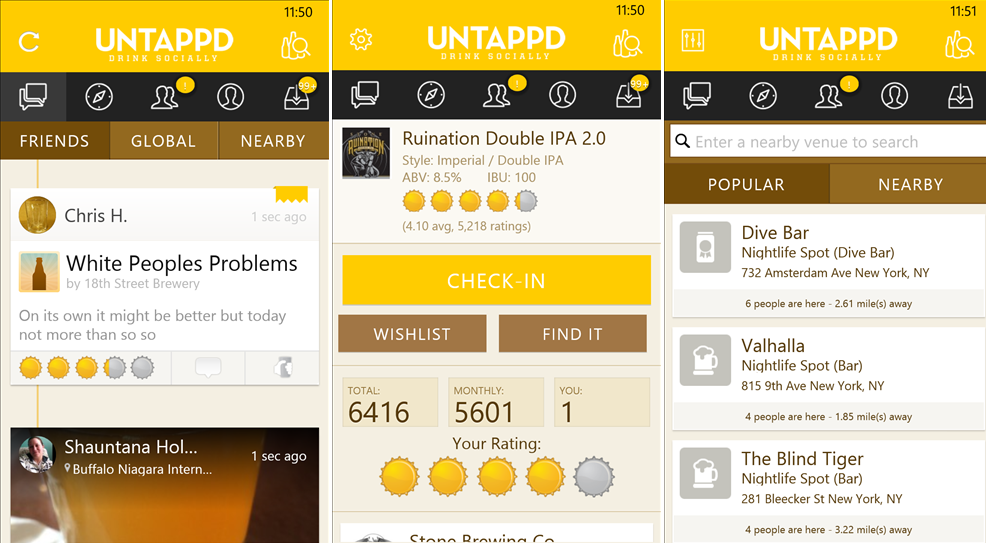
\includegraphics[width=16cm]{pictures/untapped} 
\bigbreak 

Untappd is a social network for people drinking beer.  It's main use if for
checking inn beer and sharing places with friends, and other people. Its been
growing in the later year along with the consumption of local microbreweries.
The app surpassed 1 million users in 2014 and is growing~\cite{untappd}

Untappd is specialized inn beers. It has a huge database containing hundred of
thousands different beers. This is all sorted into categories ranging from Pale
Ales too Stout and heavier bear. They also allow breweries too analyze the check
inn data and the consumption of their beers. This is a useful feature and one I
believe is one of the strengths of the applications of these kind of
applications.

The app itself is interesting. When you open the app you are introduced with
a timeline containing the last check in of your friends and acquaintances. The
menu lets you a selection of nearby beers and breweries, friend list, profile and
recent notifications. The actual check in of the app is not obvious at the first
look. The search button is placed in the upper right corner of the app, and is
tricky to get used too. The search itself feels smart. It responds well when you
enter name suggestions and it's usually correct.

There is an indication on the row if you checked in the beer before. If you
have, the rating from last time gets inserted. You can then do a reevaluation
and choose a new score if you wish. Rest of the menu is OK. There is a button to
add location and picture, along with a description. This seems natural and is a
nice addition.

The location is based off foursquare and lets you select in their ever growing
list of places. This is a neat usage of existing app infrastructure and helps
Untappd stay on their track and not deviate. By collecting locations for
people.

Untappd has this concept of badges. An example of a badge can be drinking 5
Norwegian brewed beers. This can then have a Level where the amount is increased
slightly. This helps gamify the objectives of the app, drinking beer. This is a
rather interesting concept, and rather neat. Collecting badges comes from
anything, and Untappd does not have a small collection of badges either.

The main complains about the UI is the lack of usability in certain places. The
search button is placed in a very awkward place. For the case of looking up
beers, search is OK. Vivino solves this in a different interesting way, and we
will come back to this.

Untappd is in all a great app for its purpose. The usage of social media to
create their own social network is neat, and the app feels solid.


\subsubsection{Vivino}
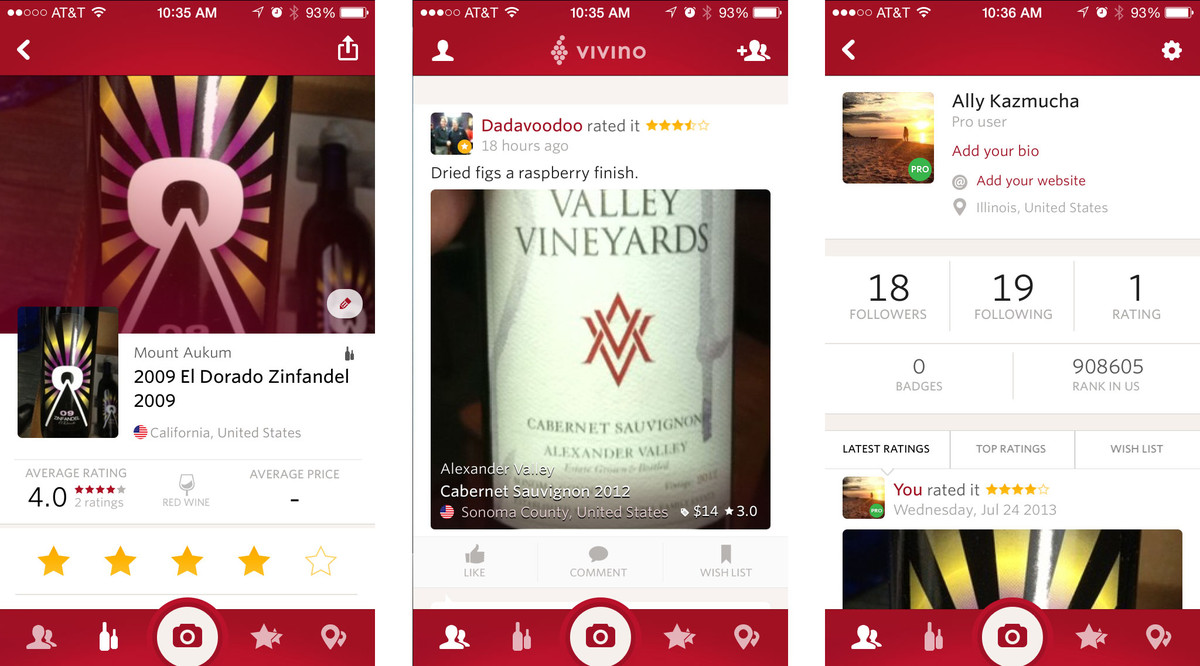
\includegraphics[width=16cm]{pictures/vivino}
\bigbreak
Vivino is a app and social network for wine. It has a lot of neat features and a
few clever ones. Vivino has of 2014 6,8 million users and a database with over 3
million different kind of wines~\cite{vivino}

While Untappd does beer, Vivino is the wine counterpart. When opening the app,
you are greeted with a timeline system. In contrast to Untappd, Vivino also
displays wine news. Lovely addition in my opinion. There are also a few notable
differences in how they approach the UI. Vivino uses the material design
principle from Google inn designing the UI. This is notable when you switch
between tabs, it moves too the direction you choose. The check in button is also
comfortable positioned at the lower right side (The picture used here is
outdated). The thumb is able to reach this place easily. Vivino lets you see the
timeline, you profile with statistics and the addition of wine recommendations.
The UI feels polished and looks great. 

The interesting part is the check in interface. The main method for checking in
wine is using a photo scanner on the label on the bottle, and it works
surprisingly well. You can also choose to take a picture of the wine menu to get
a listing, or several bottles and compare them. These features works very well
and is a neat way to check in bottles. The search part of the check in feels in
contrast rather clunky and hard to use. It's an interesting usability feature of
the app. It takes less time, its accurate enough to be more then enough.

The app then lets you rate, comment and add personal notes on the wine. You can
also see the local price on the wine and add it too a wish list. Nice addition,
and the UI again does not feel clunky or hard to use. It's responsive, it moves
very well when scrolling and the elements works well.


\subsection{Use case}
We will try and analyze the requirements for the app using Use Case
analysis\cite[p.109-113]{usecase}.  Use cases tries to break down how an app will
be used in terms of what it should do. Then you can break it further down and
analyze the requirements needed to fulfill this action. One could make fictional
personas\cite[p.108]{usecase} to try and figure out how different people would
utilize your app or website.

Personas can take different shapes. You could go along and use the app as with a
normal average user. Early 20's with the need of doing something without too
much effort. Another example could be to try use the app as a disabled person.
This could highlight potential flaws inn the design of the app that could make
it harder for a blind person to use it.

Use cases does not have a hard guideline on how it should be done. Usually you
have a graph detailing the steps needed for a feature, which you can break down
into a list. As the main feature of the app is all about searching for food and 

We will attempt this for the main feature of Forkd, the check inn. This feature
is the bread and butter of the app as a whole. It is based on the concept of
checking inn 


\bigbreak
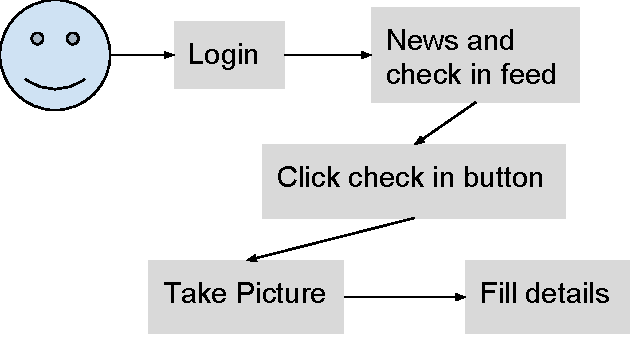
\includegraphics[width=16cm]{pictures/usecasecheckin}
\bigbreak

\textbf{Use Case:} Check in a dish

\textbf{What user:} Member (Registered User)

\begin{enumerate}[leftmargin=-0in]
  \item[] \textbf{Scenario:} 
    \begin{itemize}
      \item The member logs into the app and checks inn the dinner.
    \end{itemize}

\end{enumerate}

\begin{itemize}[leftmargin=-0in]
  \item[] \textbf{Basic flow:}

    \begin{enumerate}
      \item Logs into the app with username and password
      \item Gets presented with the feed, containing news and check inns
      \item Clicks the check inn button
      \item Gets presented with a camera screen, the user takes a photo
      \item The screen presents the photo along with a rating system, a search
        bar for location and one for dishes, and description box
      \item The user fills it inn, and approves.
      \item Check inn finished
    \end{enumerate}

\end{itemize}

There are a number of inferred requirements that comes into play here for this
app to function. These are essential for how the app works and functions to
respond too the UI.

\begin{itemize}[leftmargin=-0in]
  \item[] \textbf{Functional requirements:}
    \begin{enumerate}
      \item There should be a login mechanism
      \item The app should be able to fetch news and other check inns
      \item Use the phone camera
      \item Searching should be able to index and classify the dish 
      \item The check in needs to be stored and retrievable
    \end{enumerate}
\end{itemize}

These are all things that needs to be in order for the app to functional. The
apps needs to be able to look up the dishes and categorize them. This could help
support recommendations, catalogs of dishes and maybe even adding the recipe
later on. This isn't going to be widely discussed inn detail through this
assignment, but as mentioned earlier; the technology is there. There are
standards inn place for this too function. It does however require a great deal
of parsing, sorting and being able to reliably find dishes for the end user. I'd
argue this is a harder problem then the interaction design of this application.


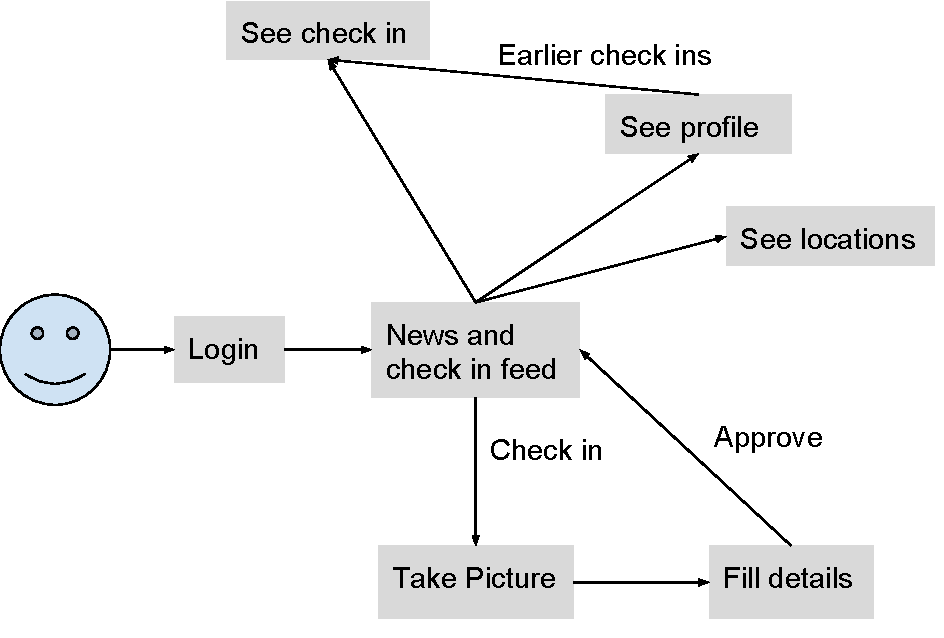
\includegraphics[width=16cm]{pictures/usecase}
\bigbreak

This shows all the possible features this app should support. We have a feed,
containing check ins and news about food. Own page for viewing a given check in,
a profile page and a location page for looking up new locations. These are all
part of what makes the app experience complete.

This is also been the basis of the development of the prototype, while the
system is simplified and the work is put into the core features of the app.


\section{Prototype}

Prototyping is the act of making an example of the given application. This
could be simple interfaces, quickly programmed application to test out the core
features of the application. These are used to check if the features of the
planned app is possible. There is no need to make it look perfect, and they
usually go through iterations. Many are as well scrapped and reworked several
times before something viable comes into play.

In this section we will take a look at the prototype designed with a tool called
FluidUI. We will see the different elements off the app come together and be
explained, and reasoned about. Does it solve the use case we defined earlier? Is
it a good starting point for the application?



\subsection{FluidUI}

FluidUI is a tool designed for quick prototyping of mobile applications and
websites. It allows people to make one free prototype with a limited feature
set, this is what I used for creating the prototype. FluidUI lets you load the
application onto your phone and test it. They also provide an example webpage
with the application running.

A link too the application at the time of writing this is found here:
\url{https://www.fluidui.com/editor/live/preview/p_4PGdVkgkGpUZnBcNIyLzA4DcXGh3sH0T.1459985039549}


\subsection{Prototype}
The prototype has a base inn the explored apps, Untappd and Vivino. They
attempt to put the social network and feed in the center of the app. In the
welcome screen. The difference as noted before is largely that Vivino attempts
to serve news and check ins, while Untappd attempts only the latter.


\subsubsection{Login view}
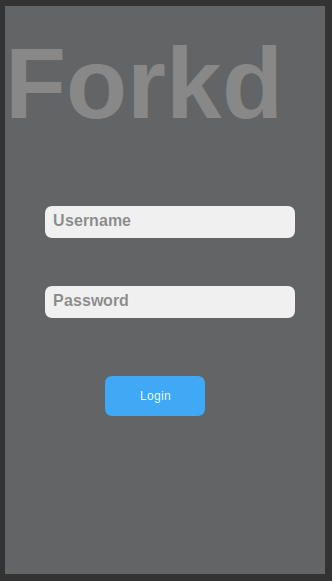
\includegraphics[width=8cm]{pictures/prototype/login}
\bigbreak

The login page is designed very straight forward. Text boxes in the center of
the screen to draw the focus there. The placement of the logo is placed there
for minimalistic reasons. It looks great and isn't in the way of the login
screen.

Optionally a login page for Facebook, twitter or other accounts could be
present. This is create features that removes the need for the user to register
on the site with yet another account. It's however omitted here as it does not
serve any purpose for the demo.


\subsubsection{List view}
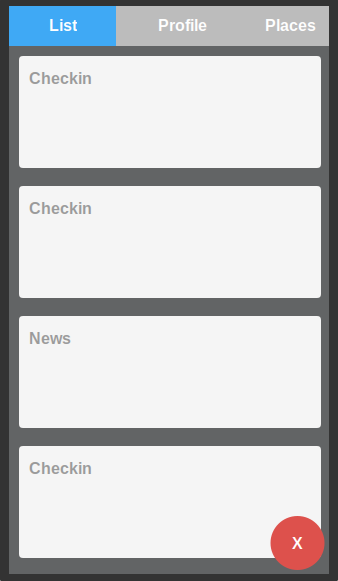
\includegraphics[width=8cm]{pictures/prototype/list}
\bigbreak

The list view is the first thing presented too the user after login. The feed
contains tiles displaying the check ins of other friends and news about dishes.
The goal of the design is to try stick with minimalism. The user does not need a
over complicated bar with a lot of options. The user does not need a search bar
on the top to search for new dishes. 

The placement of the check in button in the lower right corner is perfect. This
is pretty much taken straight out of how Vivino did their. The placement is
perfect, it is reachable by the thumb. Making it usable and not annoying. The
top bar is limited down too the essentials. The list feed, that we are currently
looking it. The profile view, where you can see your rating and former check
inns, and a location page for looking up new locations.


\subsubsection{Picture view}
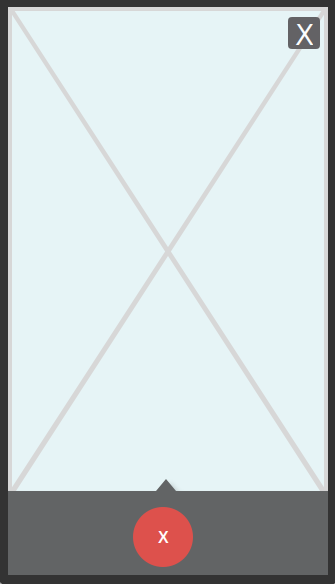
\includegraphics[width=8cm]{pictures/prototype/picture}
\bigbreak

The picture view is the first step of the check in functionality. This lets the
user take the photo of the dish in front of them. The focus here is the actual
camera display, here illustrated with the blue square. The button is an attempt
at designing a minimal design, while still leaving room for future functionality.
This could be in the form of adding effects, changing camera angel and the
likes.

We also preserve a close button in the upper right corner to exit out of the
check inn. It's simple and does not prevent the user if they intend to take a
picture. This forces them to actually reach the button and not cancel anything
by accident.


\subsubsection{Check in view}
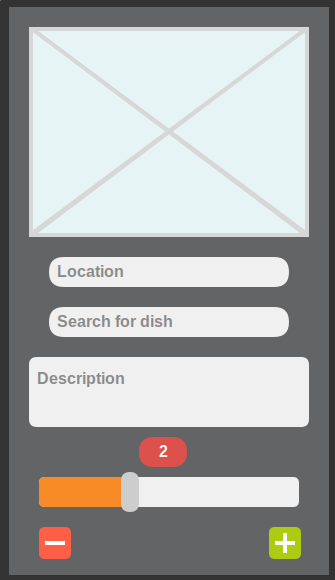
\includegraphics[width=8cm]{pictures/prototype/checkin}
\bigbreak

The check in view displays the dish after the picture is taken. You can see the
image you have just taken, search for the location you are and you can search
for the dish using the search bar.  

The location search bar would pull your location and search nearby location by a
external provider like foursquare. It's a common approach by similar apps to
outsource the information needed. Untappd does this rather successfully. This
would be able to associate the dish and the place. Making the location
retrievable and you can look up dish rating.

The dish search bar should display all the possible dishes as you search, and
allow a form of free style text search.  "Pasta dish" should return a list of
possible pasta dishes. While "Pasta Carbonara" should return the actual dish.
This could then be selected by the user and the dish is classified.

The last part is the rating system. It would let the user rather the dish from 1
too 5 using a slider for quicker access. The slider makes it easy to adjust the
score on the fly, and was the only thing available to FluidUI!

The overall design of the screen her seems a bit messy. Mostly because of the
lack of visuals and the rather bold colors with. It demonstrates the needed
components of the UI, and a lot of the problems here can be solved by enabling
scrolling.


\subsubsection{Dish view}
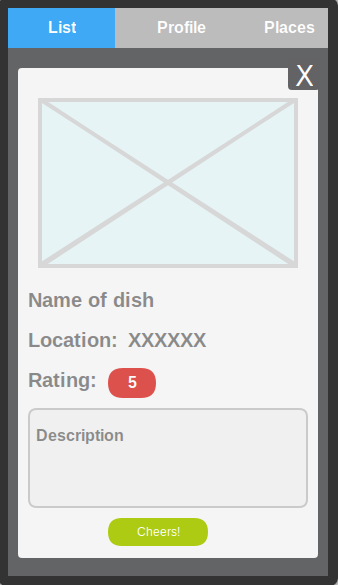
\includegraphics[width=8cm]{pictures/prototype/dish}
\bigbreak

The dish view is the main way to see a individual check in on Forkd. The view
lets you view the picture, the location and the rating of the check inn. It will
also display the description of the check in. You can vote and favor this check
in by pushing the badly named button "Cheers".

The choices made here is essentially to try and make a generalized way of
looking at dishes. The picture at the center, along with the natural flow of the
information of the dish. Giving the description most space. This could be
revised later on to adjust according too the length of the description to give
the UI more space.
 

\subsubsection{Profile view}
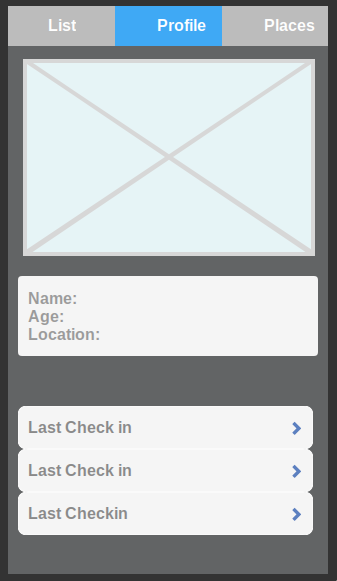
\includegraphics[width=8cm]{pictures/prototype/profile}
\bigbreak

The profile view shows your profile. It will let you scroll through the last
check inns you have registered and let you look through them and find your past
scores and check ins. The page also displays the basic information about you,
registered too your profile. This could be fetched from external social media
you choose to login with when registering.

The design is essentially designed around showing you the basic needed
information. It could probably be extended to show number of check inns in a way
Untappd or Vivino does. 


\subsubsection{Location view}
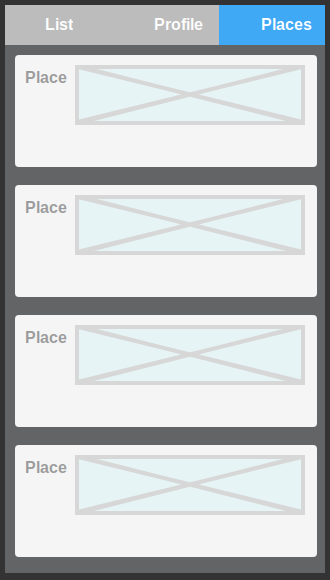
\includegraphics[width=8cm]{pictures/prototype/places}
\bigbreak

The location view lists all location in the city and gives you a picture, along
with name. Clicking on it would give you a dish menu, last rating and info about
the place. This would pull locations from foursquare and associate the dishes
along with it. This is a neat and often used way to retrieve and fetch this kind
of information.

Possible extensions would be to add a search menu, or several search options for
the location so you could narrow it further down. Untappd does this in a very
neat way. It even lets you look up local microbreweries.


\section{Evaluation}

For the evaluation I will be using the heuristics defined by Jakob Nielsen from
his book "Usability Engineering"\cite{usability}. These are 10 tests for an app to see how
usable the interface of the app is. This is not in reality a good way to test a
prototype. I was unable to gather a focus group to test and give opinions about
the app, so I believe this is an OK enough way to at least get an idea of the
design ideas behind the app.

\begin{enumerate}
  \item \textbf{Visibility of System Status}
    \begin{enumerate}
      \item [] The feedback of the app is mainly through own user interaction.
        The feed and the check in system placed at the center of the app helps
        this.
    \end{enumerate}

  \item \textbf{Match Between System and the Real World}
    \begin{enumerate}
      \item[] The app uses words such as "Check in" instead of register. You
        check in at a hotel, you don't register. It helps cultivates the user as
        a guest in the place they are.
    \end{enumerate}

  \item \textbf{User Control and Freedom}
    \begin{enumerate}
      \item[] The app contains a top bar that lets them switch between states.
        The full screen portions of the app sport a close button that lets them
        escape these places if they are missclicks.
    \end{enumerate}


  \item \textbf{Consistency and Standards}
    \begin{enumerate}
      \item[] This was mentioned earlier, but the usage of "feed", "check in",
        "profile" is well established inn the app ecosystem. Anyone using a app
        is largely familiar with the words used inn this app.
    \end{enumerate}

  \item \textbf{Error Prevention}
    \begin{enumerate}
      \item[] The UI isn't implemented, so this is hard to check. The UI tries
        to make it clear WHAT it requires from the user, in terms of input and
        interaction. Nothing is really left ambiguous with this prototype.
    \end{enumerate}

  \item \textbf{Flexibility and Efficiency of Use}
    \begin{enumerate}
      \item[] The usage of a own red check in button for check inns helps this.
        It does not require to be familiar with the app, and should be obvious.
        Ways to maybe combat this possible ambiguity is to implement a help or
        tutorial session for the app.
    \end{enumerate}

  \item \textbf{Aesthetic and Minimalist Design}
    \begin{enumerate}
      \item[] The prototype interface was largely designed to be minimalistic. Some text
        is maybe redundant, but could be completely removed if implemented in a
        clearer way. As noted there are a few exceptions where the interface
        have too much elements. This could again be resolved by scrolling.
    \end{enumerate}

  \item \textbf{Help Users Recognize, Diagnose, and Recover from Errors}
    \begin{enumerate}
      \item[] Not applicable
    \end{enumerate}

  \item \textbf{Help and Documentation}
    \begin{enumerate}
      \item[] Not applicable
    \end{enumerate}
\end{enumerate}

As noted, a few heuristics is not applicable for the prototype, as it lacks an
real implementation to be tested and actually addressed. It does however convey
some of the design choices of the app in a good way.


\section{Conclusion}
Forkd is a nice idea for an app. The technology is there, and there is enough
information to create one. There are however a few technical difficulties and
the food classification requires a lot of work. The prototype itself displays
the usage of the app in a neat way and is overall good.


\clearpage
\bibliography{oppgave}
\bibliographystyle{plain}

\end{document}
